\chapter{Hyper-parameters}\label{app:hyper}

\begin{table}[h]
\centering
\caption{Settings shared by all experiments.}
\small
\resizebox{\textwidth}{!}{%
\begin{tabular}{ll}
\toprule
item & value \\
\midrule
ground truth & DOP853, $\mathrm{rtol}=10^{-10}$, $\mathrm{atol}=10^{-12}$, grid $\tc/750$ \\
record & 4 experiments $\times\ \tfrac{20}{3}\tc$; initial-state perturbation $0.5\sigma_i$; 80/20 split \\
rollouts of learned models & classical RK4, $h=\tc/75$; divergence if $\norm{x}>10^4$ \\
model selection & rollouts of $\tc$ from 24 held-out observations; rel.\ tol.\ 5\%, abs.\ tol.\ $10^{-4}$ \\
STLSQ & 24 thresholds in $[10^{-4},10^{-0.3}]\max|\tilde\Xib_{\rm OLS}|$; ridge $10^{-10}$; $\le25$ sweeps \\
Savitzky--Golay & cubic; $w\in\{5,7,9,13,17,25\}$ \\
weak form & $\phi=(1-s^2)^4$; $H\in\{0.1,0.2,0.35,0.5,0.75\}\tc$, $H\ge2\dto$ \\
N1 network & $\tanh$, $2\times64$; output layer scaled by $0.1$ at initialisation \\
N1 training & Adam; lr $3\cdot10^{-3}$ (states $10^{-2}$), decay $0.6$/stage, cosine in last stage \\
 & batch 128 windows; clip 1; $w=0.5$; $H\in\{0.1,0.25,0.5,1\}\tc$, $\{200,250,300,450\}$ it. \\
N1 dropout (UQ) & $p=0.1$ on hidden units, mask fixed per trajectory, 30 samples \\
N2 flow-map stage & Levenberg--Marquardt, 50 it., $\mu_0=10^{-3}$, Marquardt scaling \\
N2 multiple shooting & L-BFGS (history 20, strong Wolfe), 60 it.\ per stage; $K=1,2,3,5,8,\dots,K_{\max}$ \\
 & $K_{\max}\dto\approx\tc$; $\le2048$ windows; $w=0.5$ \\
N2 thresholding & 12 values in $[10^{-3},10^{-0.4}]\max|\tilde\Xib|$; $\le4$ sweeps; L-BFGS refits (15 it., 256 windows) \\
ensembles & 5 members (N1 deep ensemble, N2 window bagging); E-SINDy 100 bootstraps \\
test sets & 16 ID + 16 OOD initial conditions; horizon 15 Lyapunov times; free runs $200\tc$ \\
\bottomrule
\end{tabular}}
\end{table}

\chapter{Additional results}\label{app:extra}

\section{Recovered equations at coarse sampling}

Lorenz-63, $\varepsilon=1\%$, seed 0 (true model: $\dot x=-10x+10y$, $\dot y=28x-y-xz$, $\dot z=-\tfrac83z+xy$).

\medskip
\noindent\textbf{$\dto=0.1$.} Weak SINDy and N2 both find the exact support at this seed. The median over seeds, $0.23$ for weak SINDy against $0.03$ for N2, reflects the other seeds.
\begin{align*}
\text{C3:}\quad & \dot x=-9.944x+9.945y,\quad \dot y=28.163x-1.074y-1.003xz,\\ & \dot z=-2.659z+0.998xy\\
\text{N2:}\quad & \dot x=-10.016x+10.060y,\quad \dot y=27.956x-1.005y-0.999xz,\\ & \dot z=-2.663z+0.997xy
\end{align*}
\noindent\textbf{$\dto=0.2$.}
\begin{align*}
\text{C3:}\quad & \dot x=-14.797x+13.943y+0.199xz-0.195yz\\
& \dot y=-24.998-7.239x+12.332y+2.864z\\
& \qquad\ +0.340xy-0.267y^2-0.236yz-0.067z^2\\
& \dot z=-57.602+8.993z+3.363x^2-2.242xy+0.595y^2-0.433z^2\\
\text{N2:}\quad & \dot x=-9.587x+9.727y-0.021xz+0.017yz\\
& \dot y=28.025x-1.018y-1.000xz,\qquad \dot z=-2.655z+1.000xy
\end{align*}
At $\dto=0.2$ the N2 model contains two spurious terms with coefficients of order $10^{-2}$, and its free runs are indistinguishable from the true attractor (\cref{fig:gallery}). The distilled N1 equations at this sampling are dense, with 26 of 30 possible terms active.

\section{Observation records in phase space}

\begin{figure}[h]
  \centering
  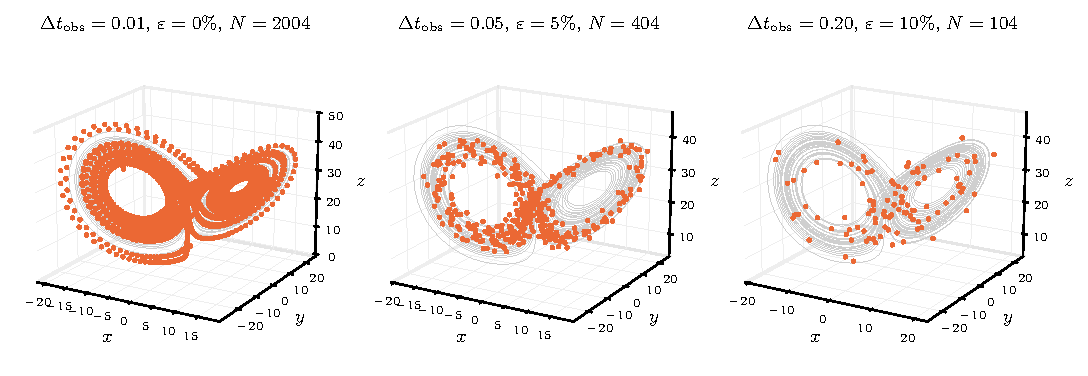
\includegraphics[width=\textwidth]{fig01_samples_phase_space}
  \caption{Lorenz-63 observations (all four experiments, seed 0) at three corruption levels, over the reference attractor.}
\end{figure}

\section{Training dynamics}

\begin{figure}[h]
  \centering
  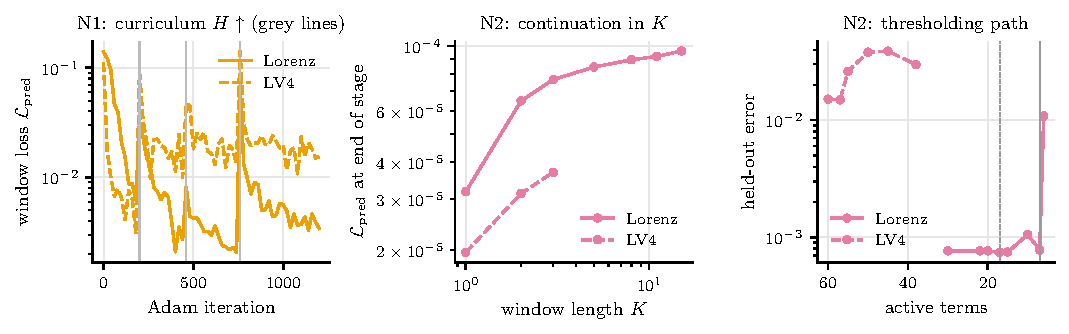
\includegraphics[width=\textwidth]{fig03_training}
  \caption{Left: N1 window loss during the curriculum ($\dto=\tc/15$, $\varepsilon=1\%$). Centre: N2 window loss at the end of each continuation stage. Right: held-out error along the N2 thresholding path; vertical lines mark the true number of active terms.}
\end{figure}
